\documentclass[tikz, convert=pdf2svg]{standalone}
\usetikzlibrary{positioning, calc, shapes}
\begin{document}
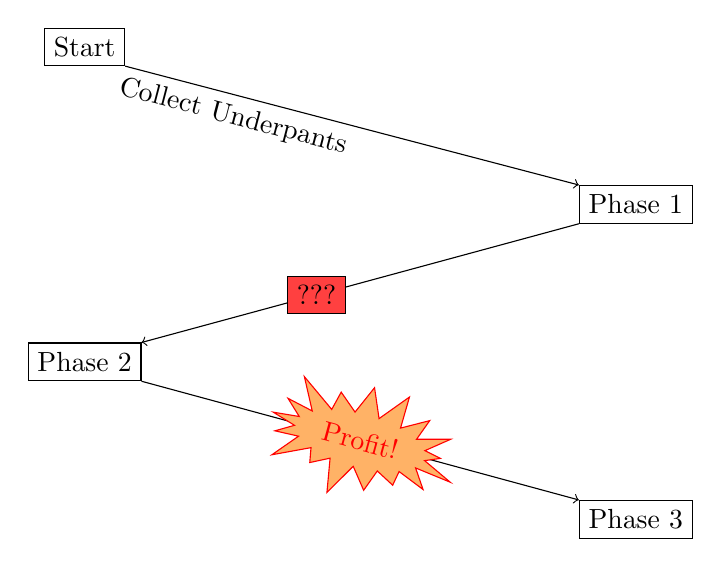
\begin{tikzpicture}

    \node[draw] (start) at (0, 8) {Start};
    \node[draw] (phase1) at (7, 6) {Phase 1};
    \node[draw] (phase2) at (0, 4) {Phase 2};
    \node[draw] (phase3) at (7, 2) {Phase 3};

    \draw[->] (start.south east) -- (phase1.north west) node[near start, below, sloped] {Collect Underpants};
    \draw[->] (phase1.south west) -- (phase2.north east) node[draw, fill=red!75, pos=0.6] {???};
    \draw[->] (phase2.south east) -- (phase3.north west) node[draw, shape=starburst, color=red, fill=orange!60, midway, sloped] {Profit!};

\end{tikzpicture}
\end{document}
